
\documentclass[11pt,a4paper,slovene]{myarticle}

%Uporabljeni paketi
\usepackage[slovene]{babel}
\usepackage[utf8]{inputenc}
\usepackage{lmodern}
\usepackage[T1]{fontenc}
\usepackage{fancyhdr}
\usepackage{caption}
\captionsetup{font={default,footnotesize}, labelfont=bf, format=hang,indention=.0cm}
\usepackage{graphicx,epsfig}
\usepackage{amsmath}
\usepackage{multirow}
\usepackage{color}
\usepackage{url}
\usepackage{makeidx}
\usepackage{listings}
\usepackage[official]{eurosym}

\definecolor{dkgreen}{rgb}{0,0.6,0}
\definecolor{gray}{rgb}{0.5,0.5,0.5}
\definecolor{mauve}{rgb}{0.58,0,0.82}

\lstset{frame=tb,
  language=C++,
  aboveskip=3mm,
  belowskip=3mm,
  showstringspaces=false,
  columns=flexible,
  basicstyle={\small\ttfamily},
  numbers=none,
  numberstyle=\tiny\color{gray},
  keywordstyle=\color{blue},
  commentstyle=\color{dkgreen},
  stringstyle=\color{mauve},
  breaklines=true,
  breakatwhitespace=true,
  tabsize=3
}

\usepackage{hyperref}
\hypersetup{
   bookmarksnumbered=true,
   urlbordercolor={0 1 0},
   linkbordercolor={1 1 1},
   unicode=true,
   pdftitle={ Modeliranje Računalniških Omrežij },
   pdfauthor={Asistent},
   pdfdisplaydoctitle=true,
   pdftoolbar=true,
   pdfmenubar=true,
   pdfstartview=X Y Z
}

\urlstyle{same}

\setlength{\parskip}{12pt}
\setlength\parindent{0pt}
\setlength\unitlength{1mm}

\begin{document}
\label{naslov}
\pdfbookmark[1]{Naslov}{naslov}
\thispagestyle{empty}

\begin{center}
\begin{Large}
Modeliranje računalniških omrežij\\
Študijsko leto 2019/2020\\
\end{Large}

\vspace*{4cm}
\begin{LARGE}
\textbf{Naloga 4 - Modeliranje IPv6 omrežij\\}
\end{LARGE}
\vspace*{0.5cm}

\begin{Large}
Poročilo za drugo seminarsko nalogo\\

\vspace*{4cm}

Mihael Šinkec\\
Vpisna št. 63170277\\
Matej Fortuna\\
Vpisna št. 63170091\\
Matej Fajdiga\\
Vpisna št. 63170084\\
Dominik Skapin\\
Vpisna št. 63150262\\

\vspace*{2cm}
Ljubljana, \today
\end{Large}
\end{center}

\pagebreak
\setcounter{page}{1}
\pagenumbering{arabic}


\label{Kazalo}
\pdfbookmark[1]{Kazalo}{Kazalo}
\tableofcontents
\thispagestyle{empty}
\pagebreak

\section{Opis primerov IPv6 omrežij}
\subsection{Omrežje 1 - IPv6 N Clients}
To omrežje je sestavljeno iz n odjemalcev, strežnika in treh IPv6 usmerjevalnikov. Strežnik nudi dostop s telnet protokolom, preko katerega odjemalci dostopajo nanj.

\begin{figure}[h]
  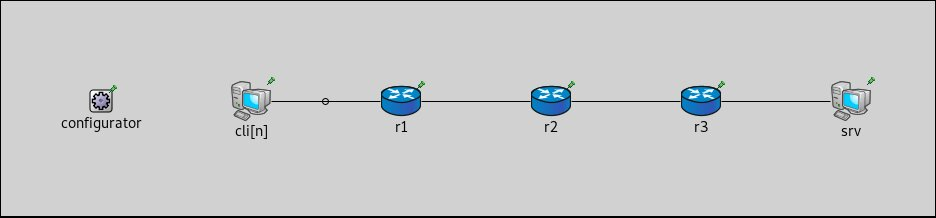
\includegraphics[width=\linewidth]{ipv6nclients.jpg}
\end{figure}

Število odjemalcev je nastavljivo preko parametra simulacije. Posameznemu odjemalcu je možno nastaviti določeno število aplikacij, ki tečejo na njem. V tem primeru na vsakemu odjemalcu teče po en telnet program/odjemalec.
telnet programu je moč tudi dodeliti poseben port. Ta je privzeto nastavljen na vrednost 1000. Nastavi se tudi IPv6 naslov strežnika, ter port telnet programa, ki teče na njem. Nato se programu nastavijo ostali parametri, kot so število poslanih ukazov, hitrost tipkanja, itd.. Primer konfiguracije izgleda takole:

\begin{lstlisting}
# tcp apps
**.cli[*].numApps = 1
**.cli[*].app[*].typename = "TelnetApp"
**.cli[*].app[0].localAddress = ""
**.cli[*].app[0].localPort = 1000
#IP address intentionally set incorrectly
**.cli[*].app[0].connectAddress = "srv[1]"
#**.cli[*].app[0].connectAddress="aaaa:2a:1:0:8aa:ff:fe00:dddd"
**.cli[*].app[0].connectPort = 1000

**.cli[*].app[0].startTime = uniform(10s,15s)
**.cli[*].app[0].numCommands = int(exponential(10))
**.cli[*].app[0].commandLength = intWithUnit(exponential(10B))
**.cli[*].app[0].keyPressDelay = exponential(0.1s)
**.cli[*].app[0].commandOutputLength = intWithUnit(exponential(40B))
**.cli[*].app[0].thinkTime = truncnormal(2s,3s)
**.cli[*].app[0].idleInterval = truncnormal(3600s,1200s)
**.cli[*].app[0].reconnectInterval = 30s
\end{lstlisting}

TODO: Opiši vrednosti

Podobno je možno konfigurirati aplikacije, ki tečejo na strežniku:
\begin{lstlisting}
**.srv[*].numApps = 1
**.srv[*].app[*].typename = "TcpGenericServerApp"
**.srv[*].app[0].localAddress = ""
**.srv[*].app[0].localPort = 1000
**.srv[*].app[0].replyDelay = 0s
\end{lstlisting}

TODO: Opiši vrednosti

Nastaviti je potrebno tudi omrežne vmesnike (NIC) na napravah:
\begin{lstlisting}
# Ethernet NIC configuration
**.eth[*].queue.typename = "EtherQosQueue"
**.eth[*].queue.dataQueue.typename = "DropTailQueue" # in routers
**.eth[*].queue.dataQueue.frameCapacity = 10  # in routers
**.eth[*].mac.duplexMode = true
\end{lstlisting}

TODO: Opiši vrednosti

Povezave (na 2. nivoju po TCP/IP) med posameznimi napravami se lahko nastavijo na Ethernet oz. na PPP protokol.
V tej implementaciji to ni možno narediti preko .ini parametrov, saj je treba v NED datoteki omrežja uvozit posebni tip povezave. Zato je potrebno ustvariti posebej NED datoteko za ethernet, kot tudi za PPP.
Tej povezavi lahko definiramo hitrost prenosa ter latenco.

Primer za ethernet:
\begin{lstlisting}
channel ethernetline extends DatarateChannel
{
    delay = 0.1us;
    datarate = 100Mbps;
}
\end{lstlisting}

Posamezne naprave nato povežemo z definirano povezavo:
\begin{lstlisting}
 connections:
        for i=0..n-1 {
            cli[i].ethg++ <--> ethernetline <--> r1.ethg++;
        }
        r1.ethg++ <--> ethernetline <--> r2.ethg++;
        r2.ethg++ <--> ethernetline <--> r3.ethg++;
        r3.ethg++ <--> ethernetline <--> srv.ethg++;
\end{lstlisting}

Ko simuliramo omrežje se simulira vse od povezavni plasti gor do aplikacijske plasti, tj. od ethernet/PPP okvirjev, do telnet paketov. Pri vizualizaciji seveda vidimo samo okvirje, ker so paketi tudi del teh okvirjev.




\subsection{Omrežje 2 - IPv6 Bulk Transfer}
Omrežje je sestavljeno iz treh odjemalcev in enega serverja, ter usmerjevalnika ki jih povezuje. Odjemalci dostopajo do serverja, komur pošiljajo pakete, ta pa jih takoj pošlje nazaj na isti port. Konfiguracija je zelo podobna prejšnjemu omrežju.
Strežnik in odjemalci so povezani z kanalom s hitrostjo 10Mb/s in zakasnitvijo 1 mikro sekunda. Omrežje ni dokončano. To piše tudi v README datoteki.

Slika omrežja:

\begin{figure}[h]
  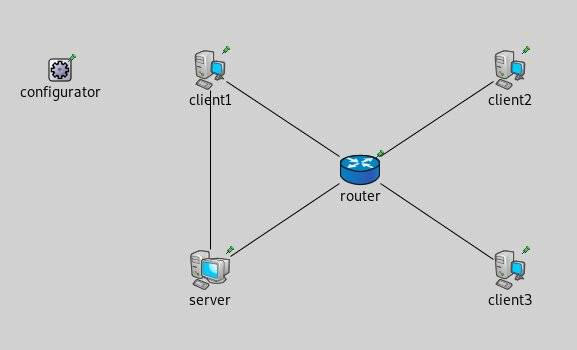
\includegraphics[width=\linewidth]{ipv6bulktransfer.jpg}
\end{figure}




\subsection{Omrežje 3 - DemoNetworkEth}
Omrežje sestavlja n odjemalcev in n strežnikov, ki med seboj komunicirajo prek dveh usmerjevalnikov.
Med napravami poteka ethernet povezava. Hitrost povezave je 10 Mb/s, zakasnitev pa je 1 mikro sekunda.

\begin{figure}[h]
  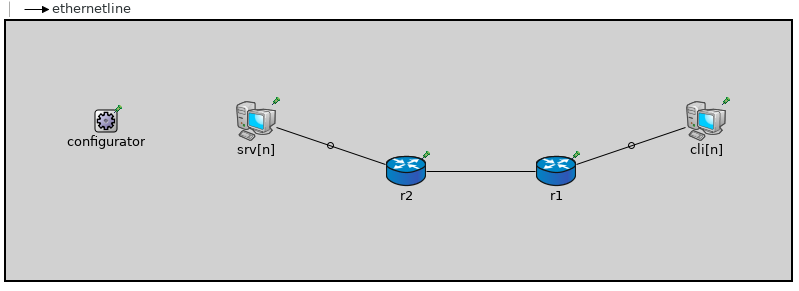
\includegraphics[width=\linewidth]{demonetworketh_struct.png}
\end{figure}



\section{Podrobna analiza enega izmed primerov: DemoNetworkEth}

Število odjemalcev in strežnikov podajamo s parametrom v .ini datoteki. Tam nastavljamo tudi ostale parametre, kot so tipi paketov (tcp/udp), število aplikacij, ki tečejo na njih in ostale.
Nastavimo lahko tudi posebna vrata. Strežniku lahko nastavimo hitrost generiranja paketov, odjemalcem pa hitrost procesiranja.

\begin{lstlisting}
# number of client and server computers
*.n = 1000      # default: *.n = 2

# configurator
#*.configurator.useTentativeAddrs=false # FIXME TBD to be switched to true, for testing DAD!

# tcp apps
**.cli[*].numApps = 1
**.cli[*].app[*].typename = "TelnetApp"
**.cli[*].app[0].localAddress = ""
**.cli[*].app[0].localPort = 1000
#IP address intentionally set incorrectly
**.cli[*].app[0].connectAddress = "srv[1]"
#**.cli[*].app[0].connectAddress="aaaa:2a:1:0:8aa:ff:fe00:dddd"
**.cli[*].app[0].connectPort = 1000

**.cli[*].app[0].startTime = uniform(10s,15s)
**.cli[*].app[0].numCommands = int(exponential(10))
**.cli[*].app[0].commandLength = intWithUnit(exponential(10B))
**.cli[*].app[0].keyPressDelay = exponential(0.1s)
**.cli[*].app[0].commandOutputLength = intWithUnit(exponential(40B))
**.cli[*].app[0].thinkTime = truncnormal(2s,3s)
**.cli[*].app[0].idleInterval = truncnormal(3600s,1200s)
**.cli[*].app[0].reconnectInterval = 30s
\end{lstlisting}

Podobno je možno konfigurirati aplikacije, ki tečejo na strežniku:
\begin{lstlisting}
**.srv[*].numApps = 1
**.srv[*].app[*].typename = "TcpGenericServerApp"
**.srv[*].app[0].localAddress = ""
**.srv[*].app[0].localPort = 1000
**.srv[*].app[0].replyDelay = 0s
\end{lstlisting}


Nastaviti je potrebno tudi omrežne vmesnike (NIC) na napravah:
\begin{lstlisting}
# Ethernet NIC configuration
**.eth[*].queue.typename = "EtherQosQueue"
**.eth[*].queue.dataQueue.typename = "DropTailQueue" # in routers
**.eth[*].queue.dataQueue.frameCapacity = 10  # in routers
**.eth[*].mac.duplexMode = true
\end{lstlisting}


Protokol pošiljanja spreminjamo v .ned datoteki. Tu definiramo tudi hitrost prenosa in latenco.

Primer za ethernet:
\begin{lstlisting}
channel ethernetline extends DatarateChannel
{
    delay = 0.1us;
    datarate = 100Mbps;
}
\end{lstlisting}

Posamezne naprave nato povežemo z definirano povezavo:
\begin{lstlisting}
 connections:
        for i=0..n-1 {
            cli[i].ethg++ <--> ethernetline <--> r1.ethg++;
            srv[i].ethg++ <--> ethernetline <--> r2.ethg++;
        }
        r1.ethg++ <--> ethernetline <--> r2.ethg++;
\end{lstlisting}

Pri simulaciji se simulirajo plasti tcp/ip modela od druge navzgor. V simulaciji pa vidimo samo okvirje.


\section{Podroben opis gradnikov, ki jih bomo uporabili v naših omrežjih}
V simulacijah bomo uporabili gradnike iz paketa "inet", ki naj bi služili simulaciji omrežnih naprav iz pravega sveta. V naši nalogo smo se osredotočili na simulacijo IPv6 omrežij.

Naprave v tem paketu so sestavljene iz posameznih komponent, ki so urejeni po TCP/IP slojih.

\begin{figure}[h]
  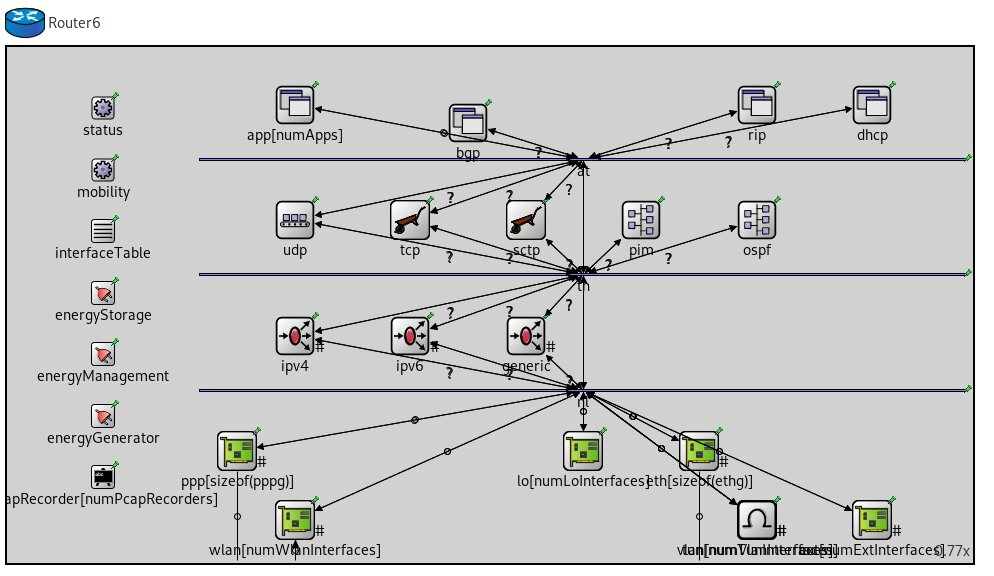
\includegraphics[width=\linewidth]{router6.jpg}
\end{figure}

Zgornji primer prikazuje sestavo naprave "Router6", ki simulira IPv6 usmerjevalnik.
Čisto spodaj se nahajajo komponente, ki simulirajo delovanje fizične ter povezovalne plasti (skupaj se imenujeta "dostopovna plast"). Ta je sestavljena iz različnih fizičnih vmesnikov, kot so Ethernet, PPP, WLAN, itd..
Nad tem so komponente za omrežno plast. Ti določajo, katere protokole iz omrežne plasti bo naprava podpirala.
Potem pride prenosna oz. transportna plast. Tam so komponente, ki določajo podoporo prenosnih protokolov, kot so TCP in UDP.
Najvišje pa je aplikacijska plast. Tam se nahaja (v odjemalcih in strežnikih) sam simuliran program, kot tudi ostali "sistemski" programi, kot je DHCP strežnik.

V napravi so še razne komponente, ki simulirajo stvari, kot so poraba energije.

\begin{figure}[h]
  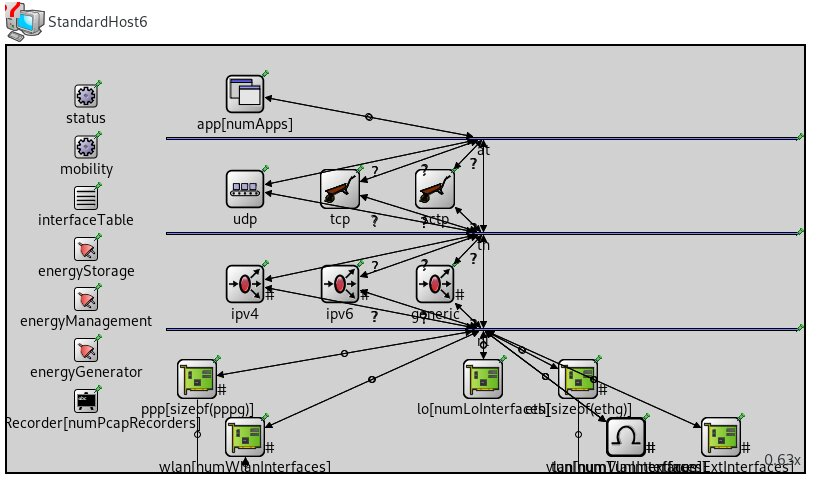
\includegraphics[width=\linewidth]{standardhost6.jpg}
\end{figure}

To je primer naprave, ki ponazarja navaden računalnik. Naprava je precej podobna usmerjevalniku, le da ji manjkaji stvari, kot so DHCP strežnik, idp.
Ta naprava se uporabi za simuliranje odjemalcev, prav tako pa tudi za simuliranje strežnikov.


\section{Gradnja in simulacija modelov IPv6 omrežij}

\subsection{Omrežje 1}
V tem omrežju se nahaja strežnik, ki ponuja TCP aplikacijo za prenos vsebin. Ta je povezan na omrežje,
na katerega so povezavni tudi odjemalci. Eden od odjemalcev je neposredno povezan na strežnik.

Med napravami so posebej konfigurirane povezave. Določljiva je kapaciteta in latenca povezave:
\begin{lstlisting}
channel C extends DatarateChannel
{
    datarate = 10Mbps;
    delay = 0.1us;
}
\end{lstlisting}


\begin{figure}[h]
  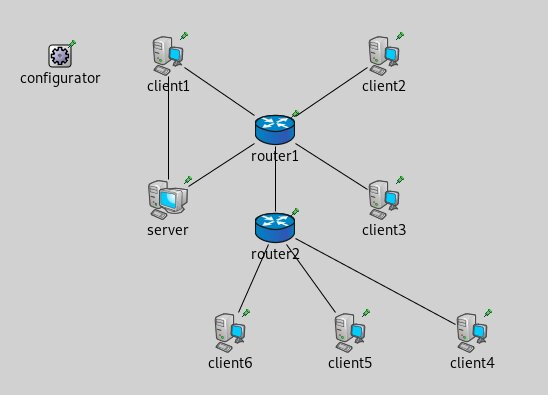
\includegraphics[width=\linewidth]{omrezje1.jpg}
\end{figure}

Povezave med napravami imajo definirano kapaciteto na 10Mb/s, ter latenco na 0,1us:
Kapaciteta povezave je definirana z 10 Mb/s, latenca pa z 0,1us.
\begin{lstlisting}
 channel C extends DatarateChannel
{
    datarate = 10Mbps;
    delay = 0.1us;
}
\end{lstlisting}

Program, ki se simulira na odjemalcih se imenuje "TcpSessionApp". S strežnikom sklene povezavo preko TCP vrat 1000. Nato pošlje 1MB podatkov strežniku:

\begin{lstlisting}
**.client*.numApps = 1
**.client*.app[*].typename = "TcpSessionApp"
**.client*.app[0].active = true
**.client*.app[0].localAddress = ""
**.client*.app[0].localPort = -1
**.client*.app[0].connectAddress = "server"
**.client*.app[0].connectPort = 1000
**.client*.app[0].tOpen = 5s
**.client*.app[0].tSend = 7s
**.client*.app[0].sendBytes = 1000000B
**.client*.app[0].sendScript = ""
**.client*.app[0].tClose = 0s

**.server.numApps = 1
**.server.app[*].typename = "TcpEchoApp"
**.server.app[0].localAddress = ""
**.server.app[0].localPort = 1000
**.server.app[0].echoFactor = 2.0
**.server.app[0].echoDelay = 0s
\end{lstlisting}

Čakalna vrsta na usmerjevalnikih ima kapaciteto 10 ethernet okvirjev. Ob primeru da je polna, zavrže novo prispele okvirje:

\begin{lstlisting}
**.eth[*].queue.typename = "EtherQosQueue"
**.eth[*].queue.dataQueue.typename = "DropTailQueue" # in routers
**.eth[*].queue.dataQueue.frameCapacity = 10  # in routers
**.eth[*].mac.duplexMode = true
\end{lstlisting}

V tem omrežju sta ključna količina prenešenih podatkov in kapaciteta povezave med odjemalcem in strežnikom. Ta dva parametra določita čas prenosa podatkov:
$čas = količina podatkov / hitrost prenosa$

V zgornjem primeru se prenese 1MB = 8Mb podatkov preko 10Mb/s povezave, torej bo prenos trajal približno 0,8s. Dejanski čas bo verjetno višji zaradi latenc in kontrolnih okvirjev, ki se morajo prenašat po povezavah.
Zraven pa še pride čas prebivanja v usmerjevalnikih.
To drži ob primeru, da samo en odjemalec prenaša po neki povezavi. Pri večih vzporednih prenosih se čas temu sorazmerno poveča.

\subsubsection{Analiza simulacije}

Konfiguracija simulacije je sledeča:

\begin{lstlisting}
network = Seminarska1_1
sim-time-limit = 1000s

**.client*.numApps = 1
**.client*.app[*].typename = "TcpSessionApp"
**.client*.app[0].active = true
**.client*.app[0].localAddress = ""
**.client*.app[0].localPort = -1

**.client*.app[0].connectAddress = "server"
**.client*.app[0].connectPort = 1000
**.client*.app[0].tOpen = 5s
**.client*.app[0].tSend = 7s
**.client*.app[0].sendBytes = 1MB
**.client*.app[0].sendScript = ""
**.client*.app[0].tClose = 1001s

**.server.numApps = 1
**.server.app[*].typename = "TcpEchoApp"
**.server.app[0].localAddress = """
**.server.app[0].localPort = 1000
**.server.app[0].echoFactor = 2.0
**.server.app[0].echoDelay = 0s

# NIC configuration
**.ppp[*].queue.typename = "DropTailQueue" # in routers
**.ppp[*].queue.frameCapacity = 10  # in routers

**.eth[*].queue.typename = "EtherQosQueue"
**.eth[*].queue.dataQueue.typename = "DropTailQueue" # in routers
**.eth[*].queue.dataQueue.frameCapacity = 10  # in routers
**.eth[*].mac.duplexMode = true

**.router1.hasTcp = false
**.router1.hasUdp = false

**.router2.hasTcp = false
**.router2.hasUdp = false
\end{lstlisting}

V tej simulaciji odjemalci vpostavjo TCP povezavo s strežnikom ob simulacijskem času 5s. Pri 7s se začne pošiljanje podatkov strežniku. Vsak odjemalec pošlje 1M podatkov strežniku, ta pa hkrati vrača ene in iste podatke posameznemu odjemalcu, torej tudi 1M.

Simulacijo smo zaključili po 60s.

Nato smo izvozili zajeto statistiko v JSON format, ter ga nato podrobneje analizirali s pomočjo Pythona.

Ključen v tem omrežju je usmerjevalnik 1, skozi katerega grejo vsi poslani podatki.

Število paketov v čakalnih vrstah posameznega Ethernet vmesnikov na usmerjevalniku skozi čas:
\begin{figure}[h]
  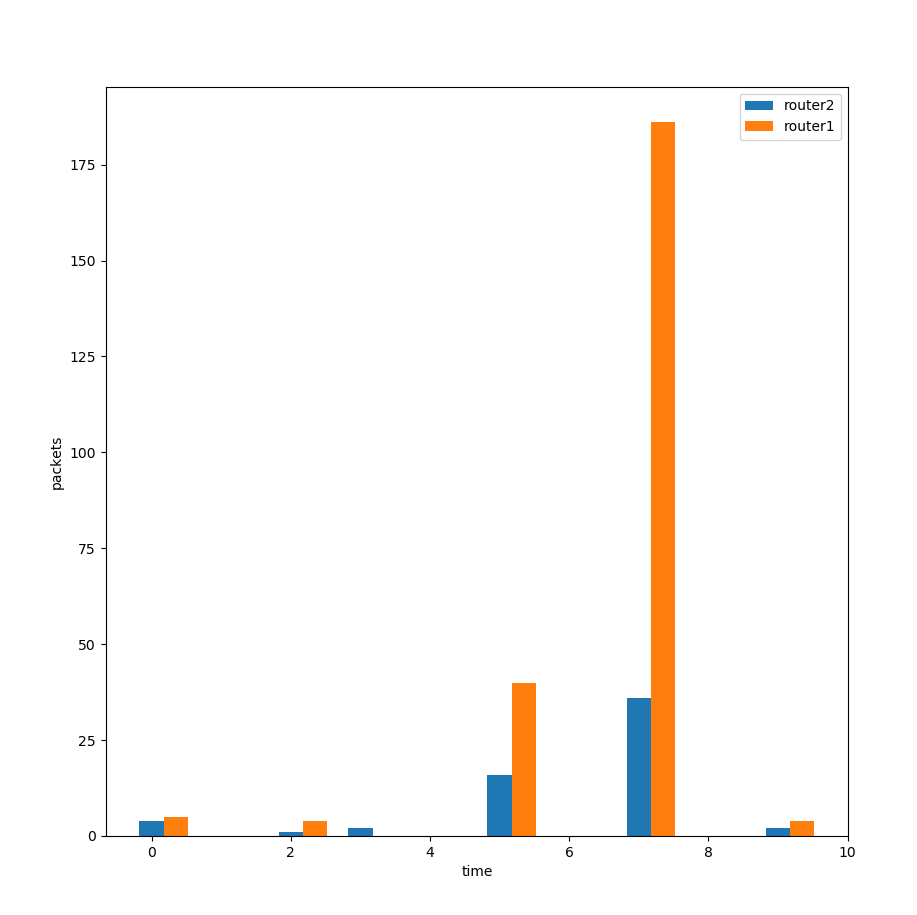
\includegraphics[width=\linewidth]{queuelength-1.png}
\end{figure}

\pagebreak

Število paketov, ki so jih obdelali usmerjevalniki:
\begin{figure}[h]
  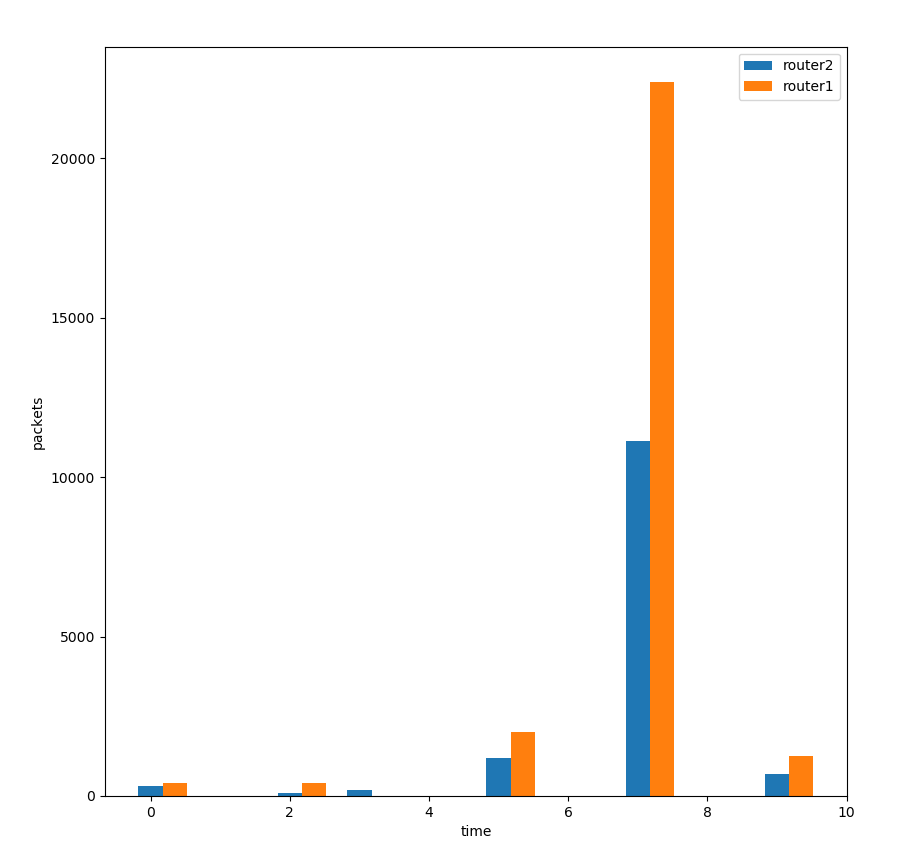
\includegraphics[width=\linewidth]{packets-1.png}
\end{figure}

\pagebreak
\subsection{Omrežje 2}
V tem omrežju je pokazana Peer to Peer omrežje med tremi računalniki in prenos podatkov skozi le to omrežje. 

Med napravami so posebej konfigurirane povezave. Določljiva je kapaciteta in latenca povezave:
Kapaciteta povezave je definirana z 10 Mb/s, latenca pa z 0,1us.

\begin{lstlisting}
channel C extends DatarateChannel
{
    datarate = 10Mbps;
    delay = 0.1us;
}
\end{lstlisting}

\begin{figure}[h]
  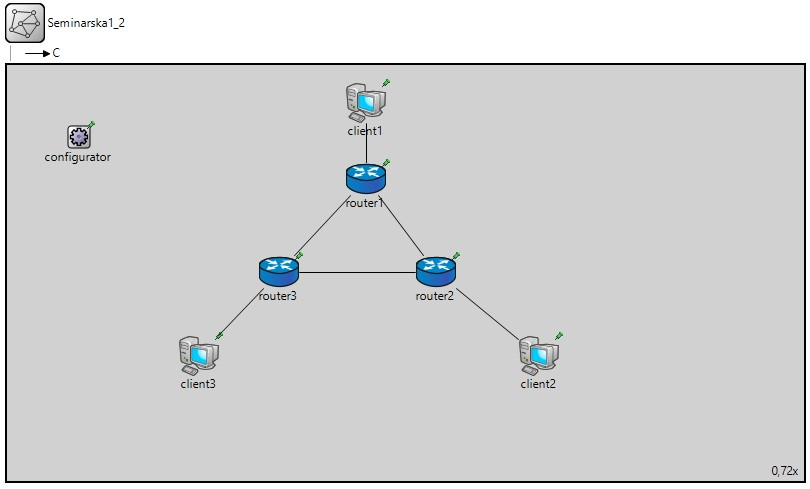
\includegraphics[width=\linewidth]{omrezje2.jpg}
\end{figure}

Programa, ki se simulirata na odjemalcij sta "TcpSessionApp" in "TcpEchoApp". Med seboj so povezani preko porta 1001 in si pošiljajo TCP paketke velikosti 10MB.

\begin{lstlisting}
**.client*.numApps = 2
**.client*.app[0].typename = "TcpSessionApp"
**.client*.app[0].localPort = 1001
**.client*.app[0].active = true
**.client*.app[0].localAddress = ""
**.client*.app[0].tOpen = 5s
**.client*.app[0].tSend = 7s
**.client*.app[0].sendBytes = 10000B
**.client*.app[0].sendScript = ""
**.client*.app[0].tClose = 51day
**.client1.app[0].connectAddress = "client2"
**.client2.app[0].connectAddress = "client3"
**.client3.app[0].connectAddress = "client1"
**.client*.app[0].connectPort = 1000

**.client*.app[1].typename = "TcpEchoApp"
**.client*.app[1].active = true
**.client*.app[1].localPort = 1000
**.client*.app[1].echoFactor = 2.0
**.client*.app[1].echoDelay = 0
**.client*.app[1].localAddress = ""
\end{lstlisting}

Čakalna vrsta na usmerjevalnikih ima kapaciteto 10 ethernet okvirjev. Ob primeru da je polna, zavrže novo prispele okvirje:
\begin{lstlisting}
**.eth[*].queue.typename = "EtherQosQueue"
**.eth[*].queue.dataQueue.typename = "DropTailQueue" # in routers
**.eth[*].queue.dataQueue.frameCapacity = 10  # in routers
**.eth[*].mac.duplexMode = true
\end{lstlisting}

V tem omrežju je bottleneck povezava med vsmerjevalniki, saj so povezani ciklično, predvidevam, da bo to vzelo največ časa.


\subsubsection{Analiza simulacije}

Konfiguracija simulacije:

\begin{lstlisting}
network = Seminarska1_2
sim-time-limit = 50day

# tcp apps
**.client*.numApps = 2
**.client*.app[1].typename = "TcpSessionApp"
**.client*.app[1].connectPort = 1000
**.client*.app[1].localPort = 1001
**.client*.app[1].active = true
**.client*.app[1].localAddress = ""
**.client*.app[1].tOpen = 5s
**.client*.app[1].tSend = 7s
**.client*.app[1].sendBytes = 1000000B
**.client*.app[1].sendScript = ""
**.client*.app[1].tClose = 51day

**.client*.app[0].typename = "TcpEchoApp"
**.client*.app[0].localPort = 1000
**.client*.app[0].echoFactor = 2.0
**.client*.app[0].echoDelay = 0s
**.client*.app[0].localAddress = ""

**.client1.app[1].connectAddress = "client2"
**.client2.app[1].connectAddress = "client3"
**.client3.app[1].connectAddress = "client1"

# NIC configuration
**.ppp[*].queue.typename = "DropTailQueue" # in routers
**.ppp[*].queue.frameCapacity = 10  # in routers

**.eth[*].queue.typename = "EtherQosQueue"
**.eth[*].queue.dataQueue.typename = "DropTailQueue" # in routers
**.eth[*].queue.dataQueue.frameCapacity = 10  # in routers
**.eth[*].mac.duplexMode = true

**.router1.hasTcp = false
**.router1.hasUdp = false

**.router2.hasTcp = false
**.router2.hasUdp = false
\end{lstlisting}

Vsak odjemalec naslednjemu pošlje po 1MB podatkov, od drugega odjemalca pa prejme 1MB in mu jih sproti vrača. Povezava se vzpostavi pri 5ih sekundah, podatki pa se začnejo prenašat pri 7s.

Simulacijo smo ugasnili po 60s.

Število paketov v čakalnih vrstah posameznega Ethernet vmesnikov na usmerjevalniku skozi čas:
\begin{figure}[h]
  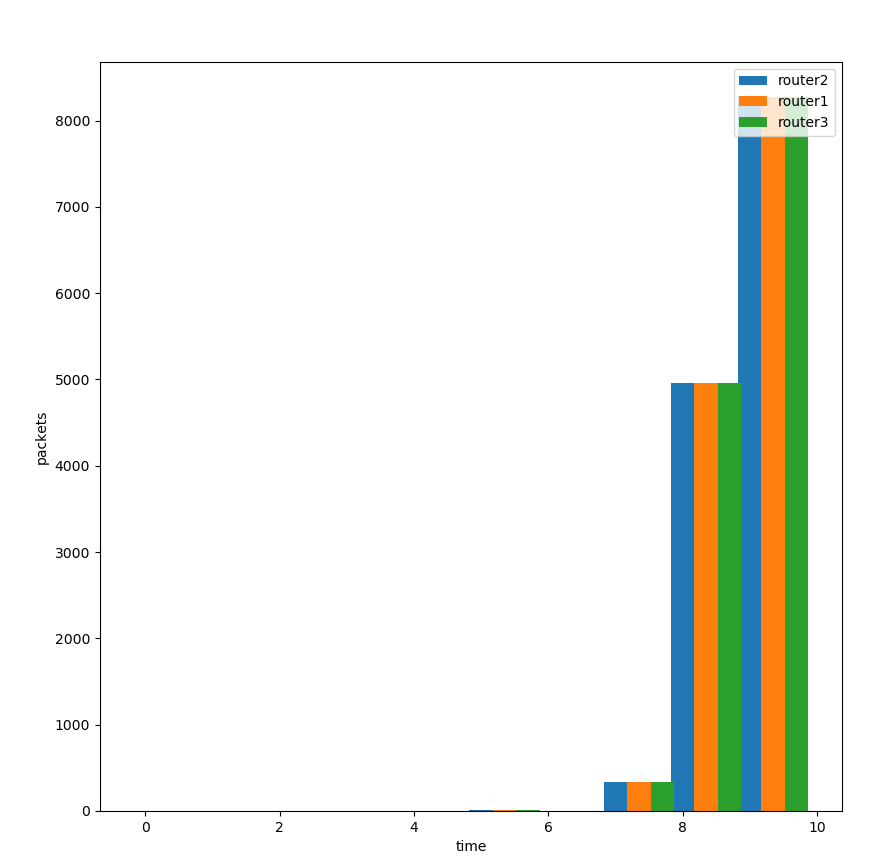
\includegraphics[width=\linewidth]{queuelength-2.png}
\end{figure}

\pagebreak

Število paketov, ki so jih obdelali usmerjevalniki:
\begin{figure}[h]
  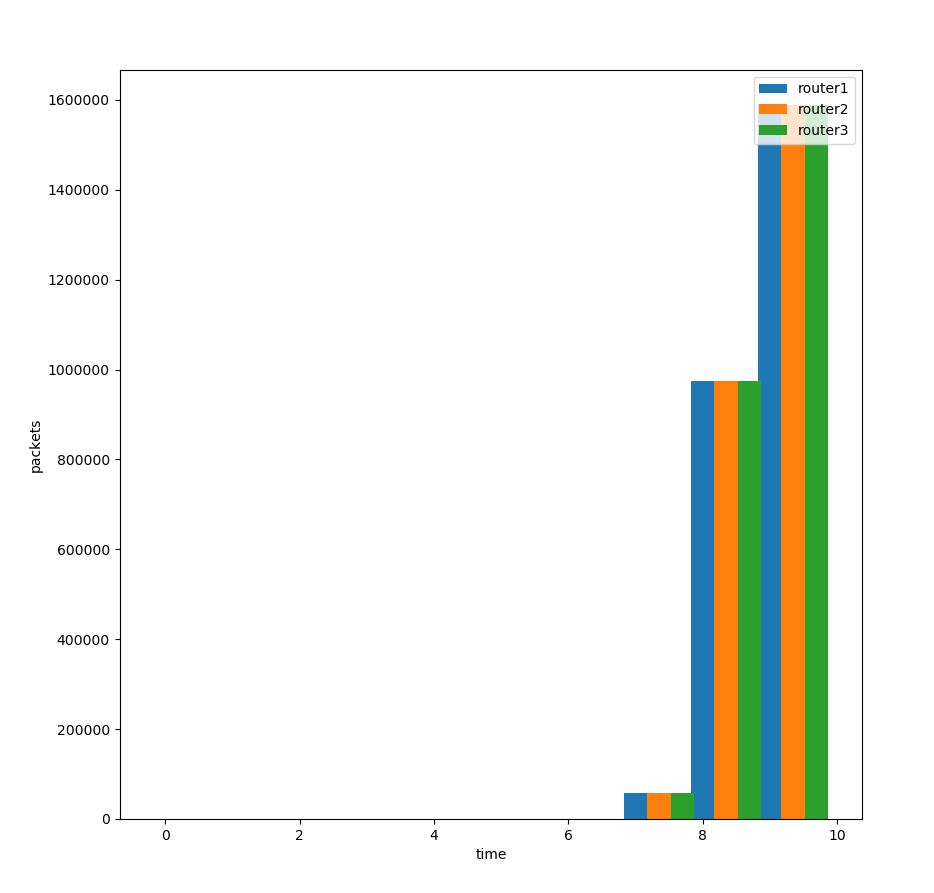
\includegraphics[width=\linewidth]{packets-2.png}
\end{figure}

\pagebreak





\subsection{Omrežje 3}
V tem omrežju je prikazana topologija zvezda. Uporablja se en strežnik, ki ponuja TCP aplikacijo za prenos vsebin. Ta je povezan na omrežje,
na katerega je povezanih n odjemalcev. Vse naprave so med seboj povezane preko usmerjevalnika.

Med napravami so posebej konfigurirane povezave. Določljiva je kapaciteta in latenca povezave:
Kapaciteta povezave je definirana z 10 Mb/s, latenca pa z 0,1us.
\begin{lstlisting}
channel C extends DatarateChannel
{
    datarate = 10Mbps;
    delay = 0.1us;
}
\end{lstlisting}

\begin{figure}[h]
  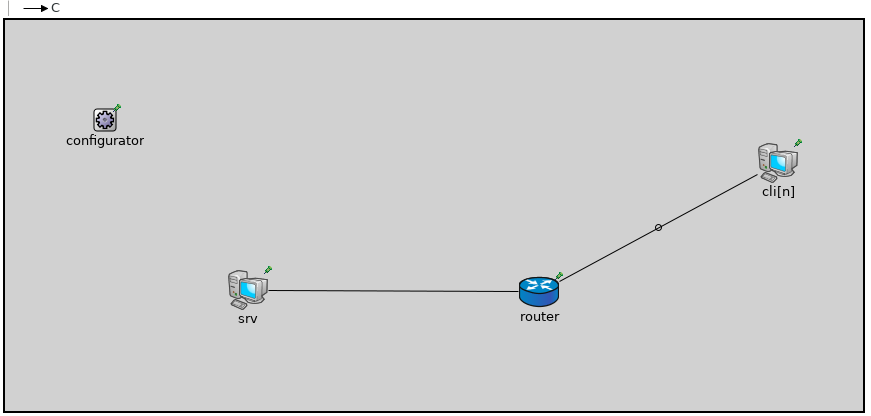
\includegraphics[width=\linewidth]{omrezje3.png}
\end{figure}

Program, ki se simulira na n odjemalcih se imenuje "TcpSessionApp". S strežnikom sklene povezavo preko TCP vrat 1000. Nato pošlje 1MB podatkov strežniku:
\begin{lstlisting}
*.n = 15

**.cli[*].numApps = 1
**.cli[*].app[*].typename = "TcpSessionApp"
**.cli[*].app[0].active = true
**.cli[*].app[0].localAddress = ""
**.cli[*].app[0].localPort = -1

**.cli[*].app[0].connectAddress = "srv"
**.cli[*].app[0].connectPort = 1000
**.cli[*].app[0].tOpen = 5s
**.cli[*].app[0].tSend = 7s
**.cli[*].app[0].sendBytes = 1000B
**.cli[*].app[0].sendScript = ""
**.cli[*].app[0].tClose = 20s

**.srv.numApps = 1
**.srv.app[*].typename = "TcpEchoApp"
**.srv.app[0].localAddress = ""
**.srv.app[0].localPort = 1000
**.srv.app[0].echoFactor = 2.0
**.srv.app[0].echoDelay = 0s
\end{lstlisting}

Čakalna vrsta na usmerjevalnikih ima kapaciteto 10 ethernet okvirjev. Ob primeru da je polna, zavrže novo prispele okvirje:
\begin{lstlisting}
**.eth[*].queue.typename = "EtherQosQueue"
**.eth[*].queue.dataQueue.typename = "DropTailQueue" # in routers
**.eth[*].queue.dataQueue.frameCapacity = 10  # in routers
**.eth[*].mac.duplexMode = true
\end{lstlisting}

V tem omrežju sta ključna količina prenešenih podatkov in kapaciteta povezave med odjemalcem in strežnikom. Ta dva parametra določita čas prenosa podatkov:
$čas = količina podatkov / hitrost prenosa$

V zgornjem primeru se prenese 1 MB = 8 Mb podatkov preko 10 Mb/s povezave, torej bo prenos trajal približno 0,8 sekunde. Dejanski čas bo verjetno višji zaradi latenc in kontrolnih okvirjev, ki se morajo prenašat po povezavah.
Poleg tega pa pride še čas prebivanja v usmerjevalniku. Tu se lahko pojavi problem, ker vse naprave komunicirajo preko enega usmerjevalnika.
Pri večjem številu paketov se časi tudi povečajo.


\subsubsection{Analiza simulacije}

Konfiguracija simulacije:

\begin{lstlisting}
network = Seminarska1_3
sim-time-limit = 50day
*.n = 15

# tcp apps
**.cli[*].numApps = 1
**.cli[*].app[*].typename = "TcpSessionApp"
**.cli[*].app[0].active = true
**.cli[*].app[0].localAddress = ""
**.cli[*].app[0].localPort = -1

**.cli[*].app[0].connectAddress = "srv"
**.cli[*].app[0].connectPort = 1000
**.cli[*].app[0].tOpen = 5s
**.cli[*].app[0].tSend = 7s
**.cli[*].app[0].sendBytes = 1000B
**.cli[*].app[0].sendScript = ""
**.cli[*].app[0].tClose = 20s

**.srv.numApps = 1
**.srv.app[*].typename = "TcpEchoApp"
**.srv.app[0].localAddress = ""
**.srv.app[0].localPort = 1000
**.srv.app[0].echoFactor = 2.0
**.srv.app[0].echoDelay = 0s

**.eth[*].queue.typename = "EtherQosQueue"
**.eth[*].queue.dataQueue.typename = "DropTailQueue" # in routers
**.eth[*].queue.dataQueue.frameCapacity = 10  # in routers
**.eth[*].mac.duplexMode = true

**.router.hasTcp = false
**.router.hasUdp = false

\end{lstlisting}

Vsak odjemalec naslednjemu pošlje po 1MB podatkov, od drugega odjemalca pa prejme 1MB in mu jih sproti vrača. Povezava se vzpostavi pri 5ih sekundah, podatki pa se začnejo prenašat pri 7s.

Simulacijo smo ugasnili po 60s.

Število paketov v čakalnih vrstah posameznega Ethernet vmesnikov na usmerjevalniku skozi čas:
\begin{figure}[h]
  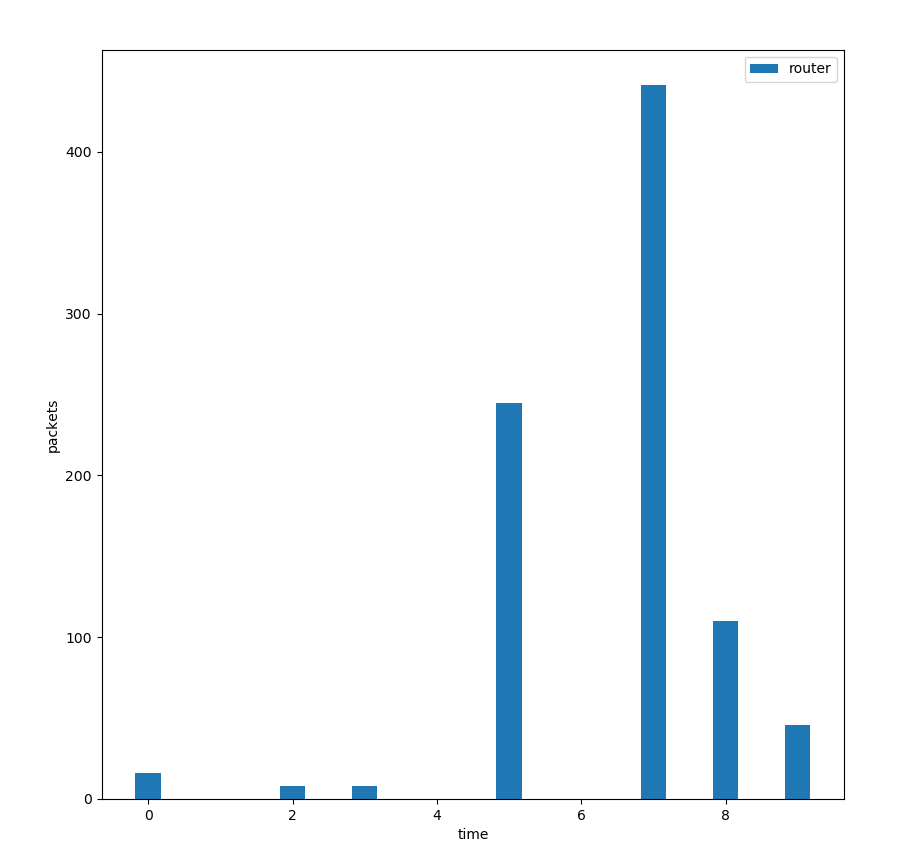
\includegraphics[width=\linewidth]{queuelength-3.png}
\end{figure}

\pagebreak

Število paketov, ki so jih obdelali usmerjevalniki:
\begin{figure}[h]
  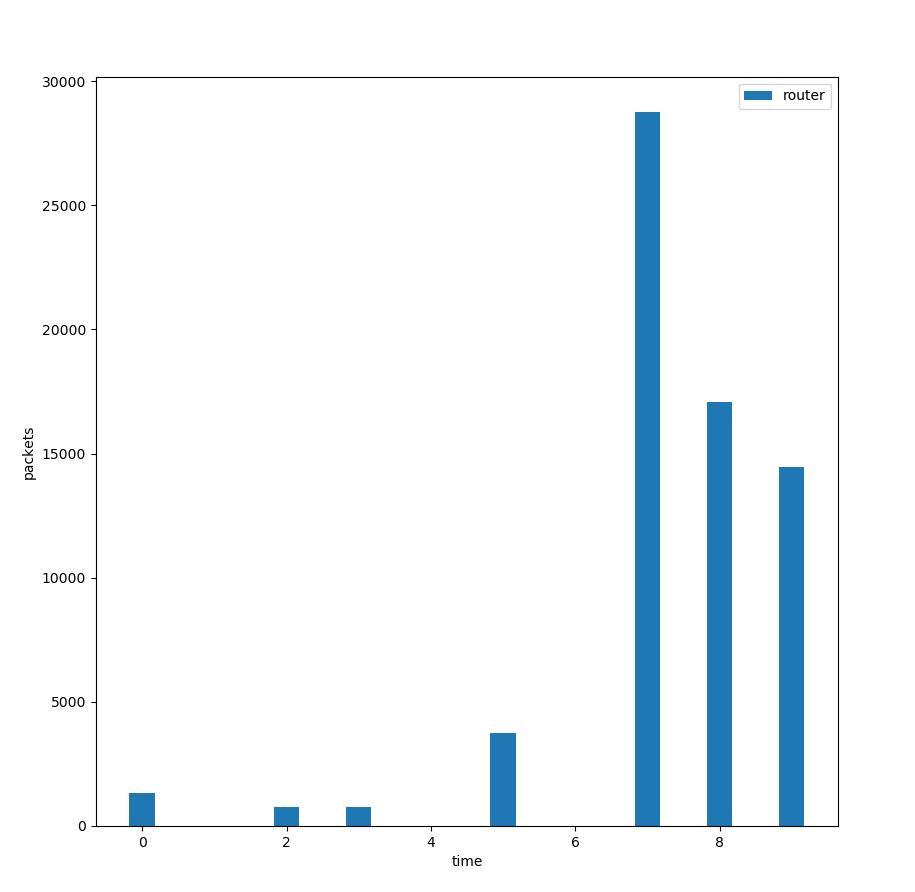
\includegraphics[width=\linewidth]{packets-3.png}
\end{figure}

\pagebreak


\subsection{Omrežje 4}
V tem omrežju je prikazana različica demonetworketh, kjer je usmerjevalnikov ravno toliko kot strežnikov/odjemalcev. Naprave so povezane tako: vsak par strežnika in odjemalca je povezan na svoj usmerjevalnik; usmerjevalniki pa so povezani med seboj v kačo. Število "n" se lahko spreminja, ponastavljeno pa je na n=2. Vsi strežniki uporabljajo TCP aplikacijo za prenos vsebin in komunicirajo vsak s svojim odjemalcem. Topologija izgleda kot nekakšen pajek.

Povezave so med vsemi napravami enake in njihova implementacija izgleda tako:
\begin{lstlisting}
channel C extends DatarateChannel
{
    datarate = 10Mbps;
    delay = 0.1us;
}
\end{lstlisting}

\begin{figure}[h]
  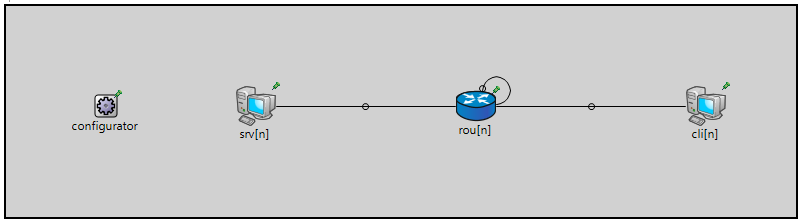
\includegraphics[width=\linewidth]{omrezje4.png}
\end{figure}

Za lepšo predstavitev, ker omnetpp usmerjevalnikov noče narisati pravilno še spodnja slika, ki prikazuje omrežje pri paramteru n=2.

\begin{figure}[h]
  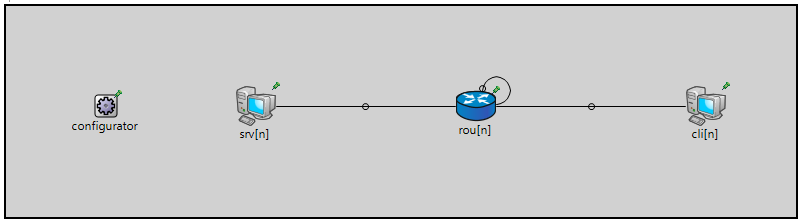
\includegraphics[width=\linewidth]{omrezje4_n_eq_2.png}
\end{figure}

Program, ki se simulira na n odjemalcih se imenuje "TcpSessionApp". S strežniki sklenejo povezavo preko TCP vrat 1000. Nato pošljejo 10MB podatkov:
\begin{lstlisting}
#number of clients, servers; default = 2
*.n = 5

# tcp apps
**.cli[*].numApps = 1
**.cli[*].app[*].typename = "TcpSessionApp"
**.cli[*].app[0].localAddress = ""
**.cli[*].app[0].localPort = 1000

#when changing *.n comment or uncomment or add below
**.cli[0].app[0].connectAddress = "srv[0]"
**.cli[1].app[0].connectAddress = "srv[1]"
**.cli[2].app[0].connectAddress = "srv[2]"
**.cli[3].app[0].connectAddress = "srv[3]"
**.cli[4].app[0].connectAddress = "srv[4]"

**.cli[*].app[0].connectPort = 1000
**.cli[*].app[0].tOpen = 5s
**.cli[*].app[0].tSend = 7s
**.cli[*].app[0].sendBytes = 10MB
**.cli[*].app[0].sendScript = ""
**.cli[*].app[0].tClose = 20s

**.srv[*].numApps = 1
**.srv[*].app[*].typename = "TcpEchoApp"
**.srv[*].app[0].localAddress = ""
**.srv[*].app[0].localPort = 1000
**.srv[*].app[0].echoFactor = 2.0
**.srv[*].app[0].echoDelay = 0s
\end{lstlisting}

Čakalna vrsta na usmerjevalnikih ima kapaciteto 10 ethernet okvirjev. Ob primeru da je polna, zavrže novo prispele okvirje:
\begin{lstlisting}
**.eth[*].queue.typename = "EtherQosQueue"
**.eth[*].queue.dataQueue.typename = "DropTailQueue" # in routers
**.eth[*].queue.dataQueue.frameCapacity = 10  # in routers
**.eth[*].mac.duplexMode = true
\end{lstlisting}


\subsubsection{Analiza simulacije}

Konfiguracija simulacije:

\begin{lstlisting}
network = Seminarska1_4
sim-time-limit = 50day

*.c = 5

*.r = 5 

# tcp apps
**.clients[*].numApps = 1
**.clients[*].app[*].typename = "TcpSessionApp"
**.clients[*].app[0].active = true
**.clients[*].app[0].localAddress = ""
**.clients[*].app[0].localPort = -1

**.clients[*].app[0].connectAddress = "server"
**.clients[*].app[0].connectPort = 1000
**.clients[*].app[0].tOpen = 5s
**.clients[*].app[0].tSend = 7s
**.clients[*].app[0].sendBytes = 1MB
**.clients[*].app[0].sendScript = ""
**.clients[*].app[0].tClose = 20s

**.server.numApps = 1
#**.server.app[*].typename="TcpSinkApp"
**.server.app[*].typename = "TcpEchoApp"
**.server.app[0].localAddress = ""
**.server.app[0].localPort = 1000
**.server.app[0].echoFactor = 2.0
**.server.app[0].echoDelay = 0s

**.ppp[*].queue.dataQueue.typename = "DropTailQueue" # in routers

**.router*.hasTcp = false
**.router*.hasUdp = false
\end{lstlisting}

Vsak odjemalec pošilje 1MB podatkov izbranemu strežniku, ki mu jih nato vrača.  TCP povezave se sklenejo ob 5s, podatki se pa začnejo pošiljati ob 7s.

Simulacijo smo zaključili ob 60s.

Število paketov v čakalnih vrstah posameznega Ethernet vmesnikov na usmerjevalniku skozi čas:
\begin{figure}[h]
  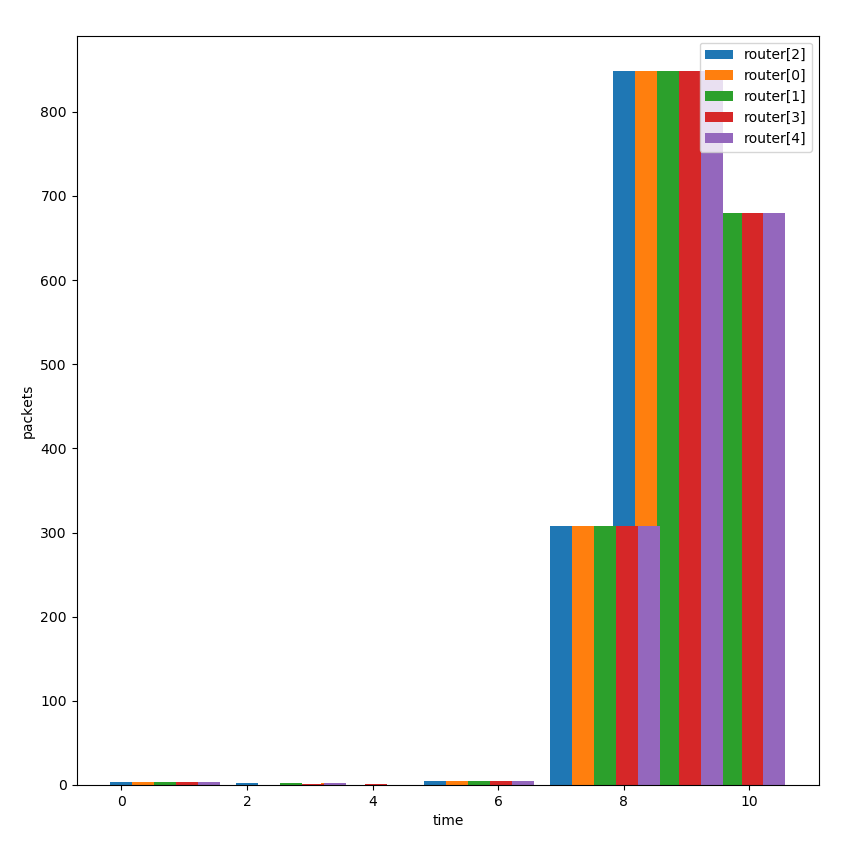
\includegraphics[width=\linewidth]{queuelength-4.png}
\end{figure}

\pagebreak

Število paketov, ki so jih obdelali usmerjevalniki:
\begin{figure}[h]
  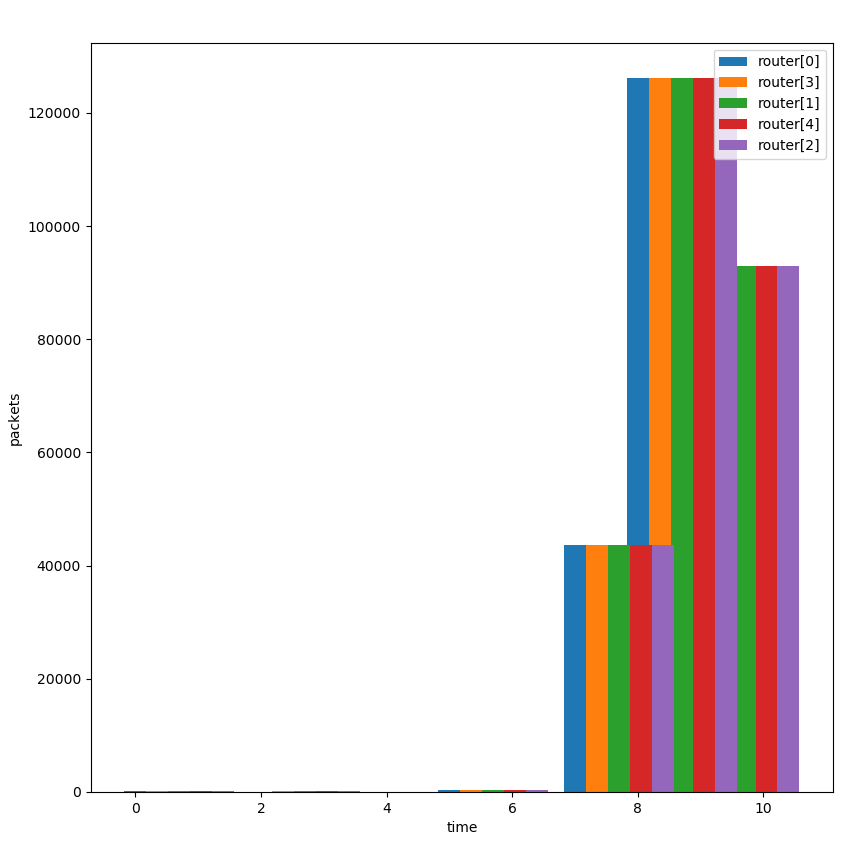
\includegraphics[width=\linewidth]{packets-4.png}
\end{figure}

\pagebreak

\end{document}

